\documentclass[12pt, a4paper]{article}
\usepackage{mathtext}
\usepackage[T2A]{fontenc}
\usepackage[utf8x]{inputenc}
\usepackage[english,russian]{babel}
\usepackage{graphicx}
\usepackage{makecell}
\usepackage{amsmath}
\usepackage{amssymb}
\usepackage{float}
\usepackage{mhchem}
\usepackage{gensymb}
\usepackage{physics}

\usepackage[a4paper,
            		left=1in,
            		right=1in,
           		 top=1in,
            		bottom=1in,
            		footskip=.25in]{geometry}

\renewcommand{\thesection}{\arabic{section}.}
\renewcommand{\thesubsection}{\arabic{section}.\arabic{subsection}.}


\title{\textbf{Отчет о выполнении лабораторной работы 2.2.3 "Измерение теплопроводности воздуха при атмосферном давлении"}}
\author{Кириченко Варвара, Б03-402}
\date{}

\begin{document}

\maketitle

\clearpage

\textbf{Цель работы:}
измерить коэффициент теплопроводности воздуха при атмосферном давлении в зависимости от температуры.
\newline


\textbf{В работе используются:}
\begin{itemize}
\item цилиндрическая колба с натянутой по оси нитью ($2r_1=50\pm3\ мкм$, $2r_0=7,0\pm0,1\ мм$, $L=400\pm2\ мм$);
\item термостат ($\sigma_{t}=0,1\ ^\circ C$);
\item вольтметр ($\varepsilon_{U}=0,012\%$) и амперметр ($\varepsilon_{I}=0,05\%$) (цифровые мультиметры);
\item источник постоянного напряжения;
\item магазин сопротивлений ($0,1\ Ом$ -- $99999,9\ Ом$)
\end{itemize}

\section{Теоретические сведения}

Теплопроводность -- это процесс передачи тепловой энергии от нагретыхчас тей системы к холодным за счёт хаотического движения частиц среды. В газах теплопроводность осуществляется за счёт непосредственной передачи кинетической энергии от быстрых молекул к медленным при их столкновениях.
Перенос тепла описывается законом Фурье, утверждающим, что плотность потока энергии $\vec{q}$ пропорциональна градиенту температуры $\nabla T$
\[\vec{q}=\kappa\nabla T\]
где $\kappa$ -- коэффициент теплопроводности. Его можно пропопрционален квадратному корню из температуры:
\[\kappa\sim\lambda\bar{v}nc_V=\frac{1}{\sigma}\sqrt{\frac{8kT}{\pi m}}\frac{i}{2}R\propto\sqrt{T}\]

В случае, когда тепло выделяется в длинном проводе, размещенном в оси полого цилиндра той же длины и теплопроводность стационарна, нетрудно получить, что тепловая мощность провода равна
\[Q=\frac{2\pi L}{\ln r_0/r_1}\kappa\Delta T\]
где $r_1$ -- радиус провода, $r_0$ -- радиус цилиндра, $L$ -- длина провода, $\Delta T$ -- перепад температуры между проводом и стенками цилиндра.

\section{Экспериментальная установка}

Схема установки приведена на рис. 1. На оси полой цилиндрической трубки с внутренним диаметром $2r_0$ размещена металлическая нить диаметром $2r_1$ и длиной $L$. Полость трубки заполнена воздухом. Стенки трубки помещены в кожух, через которых пропускается вода из термостата, так что их температура $T_0$ поддерживается постоянной.

Для измерения напряжения и тока используется два мультиметра, работающие в режимах вольтметра и амперметра соответственно. Подключение к нити $R_н$ осуществляется по четырёхпроводной схеме. По двум проводам через сопротивление пропускается измерительный ток, а два других используются для параллельного подключения вольтметра.

\begin{figure}[H]
\begin{minipage}[H]{0.5\linewidth}
\center{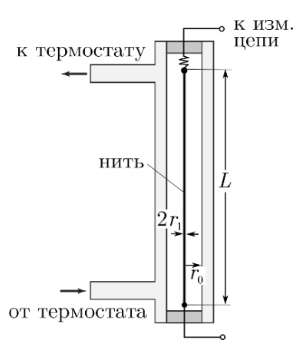
\includegraphics[width=0.7\linewidth]{223_theory2.png} \\}
\end{minipage}
\hfill
\begin{minipage}[H]{0.5\linewidth}
\center{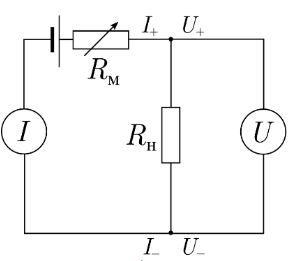
\includegraphics[width=0.7\linewidth]{223_theory1.png} \\)}
\end{minipage}
\caption{Схемы установки и цепи}
\label{ris:image1}
\end{figure}


\section{Проведение эксперимента}

\begin{enumerate}

\item Предварительно рассчитаем максимальные допустимые значения напряжения $U_{макс}$ и $I_{макс}$ тока на нити из формулы
\[Q=\frac{2\pi L}{\ln r_0/r_1}\kappa\Delta T\]
используя приближенные значения параметров установки. Получим:
\[U_{макс}=2,7\ B\quad I_{макс}=130\ mA\]

\item Выставим максимальное значение сопротивления на магазине сопротивлений. Включим вольтметр и амперметр, настроим их на нужный режим работы. Запустим источник питания и термостат.

\item Выставим на термостате комнатную температуру и будем фиксировать показания приборов, постепенно уменьшая сопротивление магазина $R_n$. Занесем данные в таблицу 2.
Значения сопротивления $R_n$ были предварительно рассчитаны таким образом, чтобы мощность, выделяемая проволокой, возрастала монотонно в диапазоне от $0$ до $Q_{max}$ (таблица 1).

\item Вновь выставим на магазине максимальное сопротивление.

\item Повторим предыдущие два пункта еще шесть раз постепенно увеличивая температуру термостата и дожидаясь ее установления.

\item Выключим все измерительные приборы, блок питания, на магазине сопротивлений установим максимальное сопротивление, а на термостате установим комнатную температуру.

\end{enumerate}
\section{Обработка данных}

\begin{enumerate}

\setcounter{enumi}{6}

\item Для каждой температуры построим зависимость $R(Q)$ ($R=\frac{U}{I},\ Q=UI$). Через точки проведем прямую МНК. Рассчитаем значения $R_0=R(0)$ и $\dv{R}{Q}$ и занесем их в таблицу 3.

\item Через точки $R_0$, полученные в предыдущем пункте, построим прямую МНК. Получим зависимость $R(T)$. Рассчитаем температурный коэффициент сопротивления нити $\alpha$ по формуле:
\[\alpha=\frac{1}{R(T_0)}\dv{R}{T},\quad T_0=273\ К\]

\item Используя результаты предыдущих пунктов, вычислим наклон зависимости выделяющейся на нити мощности $Q$ от ее перегрева $\Delta T$ относительно стенок:
\[\dv{Q}{\Delta T}=\dv{R}{T}/\dv{R}{Q}\]
Дополним таблицу 2.

\item Зная, что $\dv{Q}{\Delta T}=\frac{2\pi L}{\ln r_0/r_1}\kappa$, вычислим значение коэффициента теплопроводности $\kappa$:
\[\kappa=\frac{\ln r_0/r_1}{2\pi L}\dv{Q}{\Delta T}\]
Результаты также занесем в таблицу.

\item Построим график зависимости $\kappa(T)$ в двойной логарифмическом масштабе. Заметим, что на прямую ложатся только первые три точки, поэтому будем использовать только их. Определим показатель степени в зависимости $\kappa\propto T^\beta$.

\end{enumerate}

\section{Расчет погрешностей}

Определим относительную погрешность величин, полученных в пункте 7. Пусть зависимость $R(Q)$ имеет вид $R=kQ+b$. Тогда:
\[\varepsilon_{\dv{R}{Q}}=\sqrt{\varepsilon_{k}^2+\varepsilon_{U}^2+\varepsilon_{I}^2}=0,9\%\]
\[\varepsilon_{R_0}=\sqrt{\varepsilon_{b}^2+\varepsilon_{U}^2+\varepsilon_{I}^2}=0,08\%\]

Определим погрешность $\dv{R}{T}$ из МНК:
\[\varepsilon_{\dv{R}{T}}=\sqrt{\varepsilon_{k}^2+\varepsilon_{R_0}^2+\varepsilon_{t}^2}=2,0\%\]

Величина $1/\varepsilon_{\dv{R}{T}}\approx50$ удовлетворяет критерию Стьюдента при $n-k-1=1$ и $p=0,95$, равному 12,7.

Погрешность величины $\alpha$ выражается по формуле:
\[\varepsilon_{\alpha}=\sqrt{\frac{\sigma_k^2 T_0^2+\sigma_b^2}{(kT_0+b)^2}+\varepsilon_{\dv{R}{T}}^2}=2,0\%\]
\[\alpha=3,2\pm0,01\ \frac{10^{-3}}{К}\]

Найдем погрешность $\dv{Q}{\Delta T}$:
\[\varepsilon_{\dv{Q}{\Delta T}}=\sqrt{\varepsilon_{\dv{R}{Q}}^2 + \varepsilon_{\dv{R}{T}}^2}=2,2\%\]

Вычислим погрешность коэффициента теплопроводности:
\[\varepsilon_{\kappa}=\sqrt{\frac{\varepsilon_{r_0}^2+\varepsilon_{r_1}^2}{\ln^2(r_0/r_1)}+\varepsilon_{L}^2+\varepsilon_{\dv{Q}{\Delta T}}^2}=2,6\%\]

Наконец, определим погрешность коэффициента $\beta$:
\[\frac{\sigma_{\beta}}{\beta}=\frac{1}{\beta}\sqrt{\varepsilon_{\kappa}^2+\varepsilon_{t}^2+\sigma_{k}^2}=13\%\]
\[\beta=0.27\pm0.06\]

\section{Вывод}

В результате работы, несмотря на осложнения, вызванные данными, полученными при высоких температурах термостата, получилось определить температурный коэффициент  сопротивления платины $\alpha$, приближенный к его действительному значению $=3,9\cdot10^{-3}\ \frac{1}{К}$. Однако коэффициент $\beta$ сильно отличнается от настоящего значения, равного $=0,5$.

\section{Приложения}

\begin{table}[H]
\centering
\makebox[\textwidth][c] {
\begin{tabular}{| c | c | c | c | c | c | c | c | c | c | c | c |}
\hline
$\eta$ & 0,01 & 0,1 & 0,2 & 0,3 & 0,4 & 0,5 & 0,6 & 0,7 & 0,8 & 0,9 & 1 \\
\hline
$R_м,\ Ом$ & 207 & 50 & 28,4 & 19 & 13,4 & 9,5 & 6,7 & 4,5 & 2,7 & 1,2 & 0 \\
\hline
\end{tabular}
}
\caption{Значения $R_м$, подобранные для монотонного возрастания мощности, выделяемой нитью ($Q=\eta\cdot Q_{макс}$)}
\end{table}


\begin{table}[H]
\centering
\caption{Результаты измерений и вычислений}
\label{table:results_1}
\begin{tabular}{|c|c|c|c|c|c|c|c|c|c|c|c|}
\hline
$T$, $^\circ$C   & \multicolumn{11}{c|}{23}                                           \\ \hline
$U$, V   & 0,31  & 0,98  & 1,37  & 1,67  & 1,91  & 2,1  & 2,3  & 2,51 & 2,6 & 3,32 & 3,5 \\ \hline
$I$, A   & 0,015  & 0,047  & 0,065  & 0,077  & 0,088 & 0,096  & 0,104 & 0,111 & 0,113 & 0,143 & 0,15 \\ \hline
$R$, $\Omega$ & 20,6  & 20,9  & 21,1 & 21,6 & 21,7 & 21,9 & 22,1 & 22,6 & 23,0 & 23,2 & 23,3 \\ \hline
$Q$, W    & 0,004  & 0,046  & 0,091  & 0,131  & 0,168  & 0,202  & 0,239 & 0,279 & 0,2938 & 0,474 & 0,525  \\ \hline
\multicolumn{12}{|c|}{}                                                        \\ \hline
$T$, $^\circ$C   & \multicolumn{11}{c|}{30}                                           \\ \hline
$U$, V   & 0,32  & 1,01  & 1,38  & 1,67  & 1,92 & 2,14  & 2,31 & 2,47 & 2,62 & 3,33 & 3,5  \\ \hline
$I$, A   & 0,015  & 0,047  & 0,064  & 0,076  & 0,087  & 0,095  & 0,102 & 0,109 & 0,115 & 0,14 & 0,15 \\ \hline
$R$, $\Omega$ & 21,3 & 21,4 & 21,5 & 21,9 & 22,0 & 22,5 & 22,6 & 22,6 & 22,7 & 23,7 & 23,8 \\ \hline
$Q$, W    & 0,0048  & 0,047  & 0,088  & 0,127  & 0,167  & 0,203  & 0,236 & 0,262 & 0,301 & 0,466 & 0,515 \\ \hline
\multicolumn{12}{|c|}{}                                                        \\ \hline
$T$, $^\circ$C   & \multicolumn{11}{c|}{40}                                           \\ \hline
$U$, V   & 0,33  & 1,03  & 1,42  & 1,72  & 1,96  & 2,16  &  2,34 & 2,5 & 2,64 & 2,78 & 3,5 \\ \hline
$I$, A   & 0,015  & 0,046  & 0,063  & 0,076  & 0,086  & 0,094  & 0,101 & 0,107 & 0,113 & 0,118 & 0,143\\ \hline
$R$, $\Omega$ & 22 & 22,4 & 22,5 & 22,6 & 22,8 & 22,9 & 23 & 23,3 & 23,4 & 23,5 & 24,47 \\ \hline
$Q$, W    & 0,00495  & 0,0474  & 0,0894  & 0,131  & 0,168  & 0,203  & 0,236 & 0,267 & 0,291 & 0,328 & 0,501  \\ \hline
\multicolumn{12}{|c|}{}                                                        \\ \hline
$T$, $^\circ$C   & \multicolumn{11}{c|}{50}                                           \\ \hline
$U$, V   & 0,34  & 1,05  & 1,45  & 1,74  & 1,98  & 2,1  & 2,4 & 2,5 & 2,6 & 2,8 & 2,9 \\ \hline
$I$, A   & 0,015  & 0,046  & 0,062  & 0,074  & 0,084  & 0,092  & 0,099 & 0,103 & 0,106 & 0,113 & 0,117\\ \hline
$R$, $\Omega$ & 22,6 & 22,8 & 23,3 & 23,5 & 23,6 & 23,8 & 24,2 & 24,3 & 24,5 & 24,7 & 24,8 \\ \hline
$Q$, W    & 0,0051  & 0,048  & 0,0899  & 0,128  & 0,166  & 0,185  & 0,237 & 0,257 & 0,275 & 0,316 & 0,339\\ \hline
\multicolumn{12}{|c|}{}                                                        \\ \hline
$T$, $^\circ$C   & \multicolumn{11}{c|}{60}                                           \\ \hline
$U$, V   & 0,35  & 1,07  & 1,47  & 1,77  & 2,01  & 2,21  & 2,38 & 2,54 & 2,68 & 2,81 & 2,92 \\ \hline
$I$, A   & 0,015  & 0,045  & 0,0618  & 0,073  & 0,083  & 0,089  & 0,095 & 0,106 & 0,11 & 0,113 & 0,114\\ \hline
$R$, $\Omega$ & 23,3 & 23,7 & 23,8 & 24,2 & 24,5 & 24,8 & 25,05 & 25,1 & 25,2 & 25,5 & 25,6 \\ \hline
$Q$, W    & 0,0052  & 0,0481  & 0,0908  & 0,1292  & 0,1648  & 0,1966  & 0,226 & 0,256 & 0,284 & 0,309 & 0,332\\ \hline
\multicolumn{12}{|c|}{}                                                        \\ \hline
$T$, $^\circ$C   & \multicolumn{11}{c|}{70}                                           \\ \hline
$U$, V   & 0,36  & 1,09  & 1,5  & 1,78  & 2,03  & 2,23  & 2,4 & 2,56 & 2,7 & 2,83 & 2,94\\ \hline
$I$, A   & 0,015  & 0,045  & 0,061  & 0,072  & 0,082  & 0,089  & 0,095 & 0,101 & 0,106 & 0,11 & 0,114\\ \hline
$R$, $\Omega$ & 24 & 24,2 & 24,5 & 24,7 & 24,75 & 25,32 & 25.26 & 25,3 & 25,4 & 25,72 & 25,8\\ \hline
$Q$, W    & 0,0054  & 0,049  & 0,0915  & 0,128  & 0,166  & 0,214  & 0,228 & 0,258 & 0,286 & 0,311 & 0,335\\ \hline
\end{tabular}
\end{table}

\begin{table}[H]
\centering
\makebox[\textwidth][c] {
\begin{tabular}{| c | c | c | c | c | c | c |}
\hline
$t,\ ^\circ C$ & 23 & 30 & 40 & 50 & 60 & 70 \\
\hline
$R_0,\ Ом$ & 20,78 & 21,22 & 22,02 & 22,57 & 23,29 & 23,97 \\
$\dv{R}{Q},\ Ом/мВт$ & 5,43 & 5,21 & 4,69 & 6,73 & 7,09 & 5,44 \\
$\dv{Q}{\Delta T},\ мВт/К$ & 12,4 & 13,0 & 14,4 & 10,07 & 9,55 & 12,45 \\
$\kappa,\ мВт/(м\cdot К)$ & 24,4 & 25,6 & 28.3 & 19,8 & 18,8 & 24,5 \\
\hline
\end{tabular}
}
\caption{Значения параметров для различных температур}
\end{table}


\begin{figure}[H]
\centering
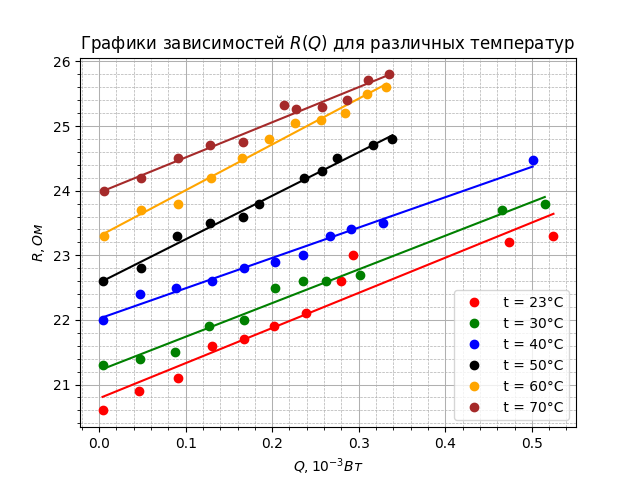
\includegraphics[width=\textwidth]{223_1.png}
\caption{Графики зависимостей $R(Q)$ для различных температур}
\end{figure}


\begin{figure}[H]
\centering
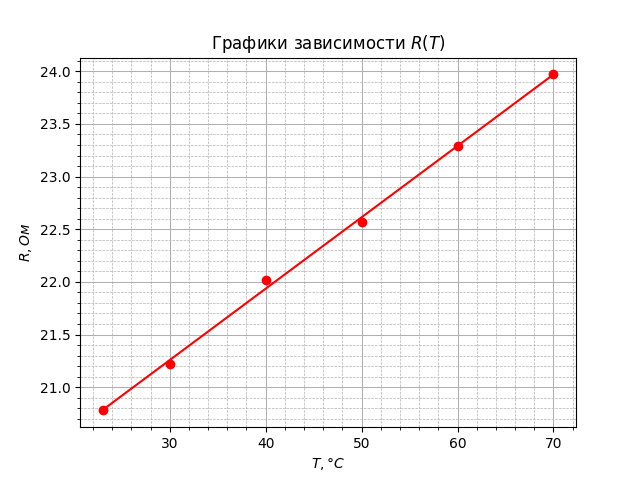
\includegraphics[width=\textwidth]{223_2.png}
\caption{Графики зависимости $R(T)$}
\end{figure}

\begin{figure}[H]
\centering
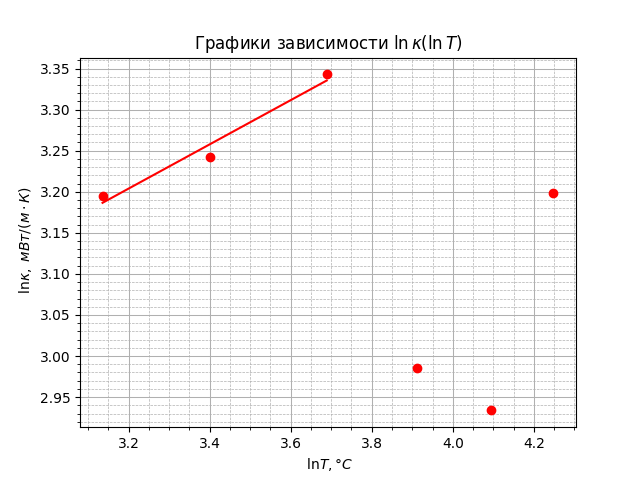
\includegraphics[width=\textwidth]{223_3.png}
\caption{Графики зависимости $\ln\kappa(\ln T)$}
\end{figure}

\end{document}

